\documentclass{beamer}
\usepackage[utf8]{inputenc}
\usecolortheme{beaver}
\usepackage{graphicx}
\usetheme{CambridgeUS}
\newcommand\tab[1][1cm]{\hspace*{#1}}


%Information to be included in the title page:
\title{Recreational Marijuana Legalization on Traffic Fatalities: Early Evidence from FARS}
\author{Nhat Hoang Pham	}
\institute{UC Denver}
\date{\today}



\begin{document}

\frame{\titlepage}

\begin{frame} % Slide 1
\frametitle{Research Question}
	What is the effect of Recreational Marijuana Legalization (RML)  on Traffic Fatalities at the state level? 
\end{frame} 
\begin{frame} % Slide 2
\frametitle{Motivation- Why RML ?}
	\begin{enumerate}
		\item
	Policy makers rely on evidence produced from medical marijuana laws (MMLs) research to inform them the effect of marijuana on public. 
		\item 
	However, RMLs can be very different from MMLs : target population, RML states already had MML \pause
		\item
	RML is a recent phenomenon, the chance that this paper get published is much higher. 
	\end{enumerate} 
\end{frame} 

\begin{frame} % Slide 2
\frametitle{Literature Review}
	\begin{itemize}
	
		\item 
		Hansen, Benjamin, Keaton Miller, and Caroline Weber. 2020a. “Early Evidence on Recreational Marijuana Legalization and Traffic Fatalities.” Economic Inquiry, 58(2): 547-568. \pause
		
		\item
		Santaella-Tenorio, Julian, Katherine Wheeler-Martin, Charles J. DiMaggio, Alvaro Castillo-Carniglia, Katherine M. Keyes, Deborah Hasin, and Magdalena Cerdá. 2020. “Association of Recreational Cannabis Laws in Colorado and Washington State with Changes in Traffic Fatalities, 2005-2017.” JAMA Internal Medicine, 180(8): 1061-1068. \pause
		
		\item
		Aydelotte, Jayson D., Lawrence H. Brown, Kevin M. Luftman, Alexandra L. Mardock, Pedro G. R. Teixeira, Ben Coopwood, and Carlos V. R. Brown. 2017. “Crash Fatality Rates After Recreational Marijuana Legalization in Washington and Colorado.” American Journal of Public Health, 107(8): 1329- 1331. \pause
		
	\end{itemize}
\end{frame} 

\begin{frame} % Slide 3
\frametitle{Data at State-Year Level(2010-2019)}
	\begin{itemize}
	
		\item
		FARS from 2010-2019 using accident, accident auxiliary, and person data files
		\item
		U.S census: population, median age, male/female population
		\item
		BEA: Income by state
		\item
		BLS: Unemployment Rate
		\item
		Highway statistics: Number of licensed driver, Vehicle miles driven 		
		\item
		National Highway Traffic Safety Administration and National Conference of State Legislatures: laws such as primary seat belts, texting ban etc. 
		\item 
		Use 10 states legalizing recreational marijuana before 2020
		
	\end{itemize}
\end{frame} 

\begin{frame} % Slide 4
\frametitle{Summary Statistics}

	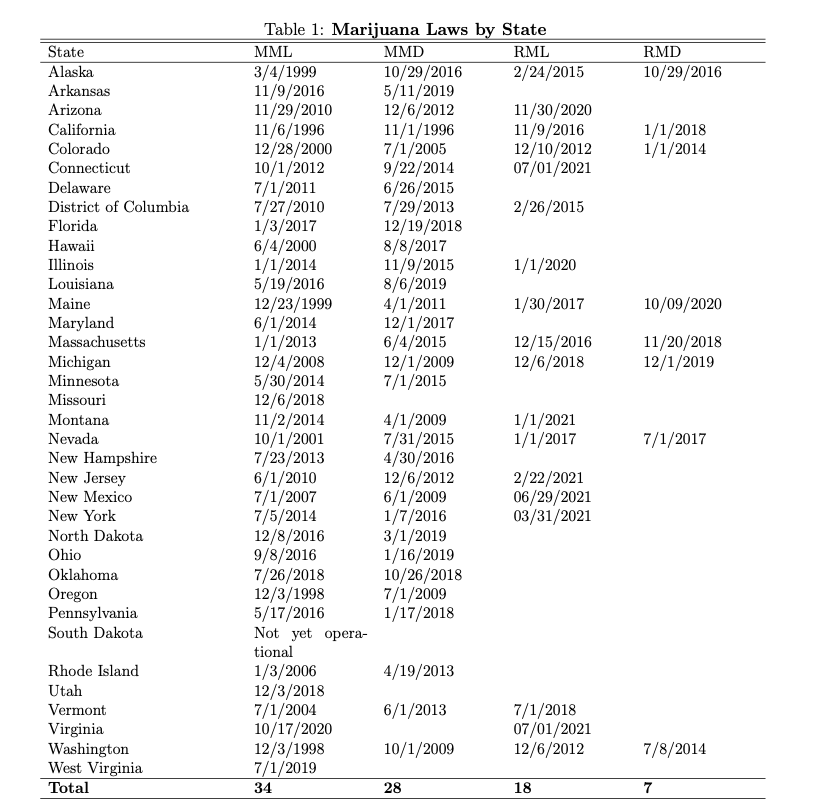
\includegraphics[scale = 0.25]{table1}

\end{frame}

\begin{frame} % Slide 4
\frametitle{Summary Statistics}

	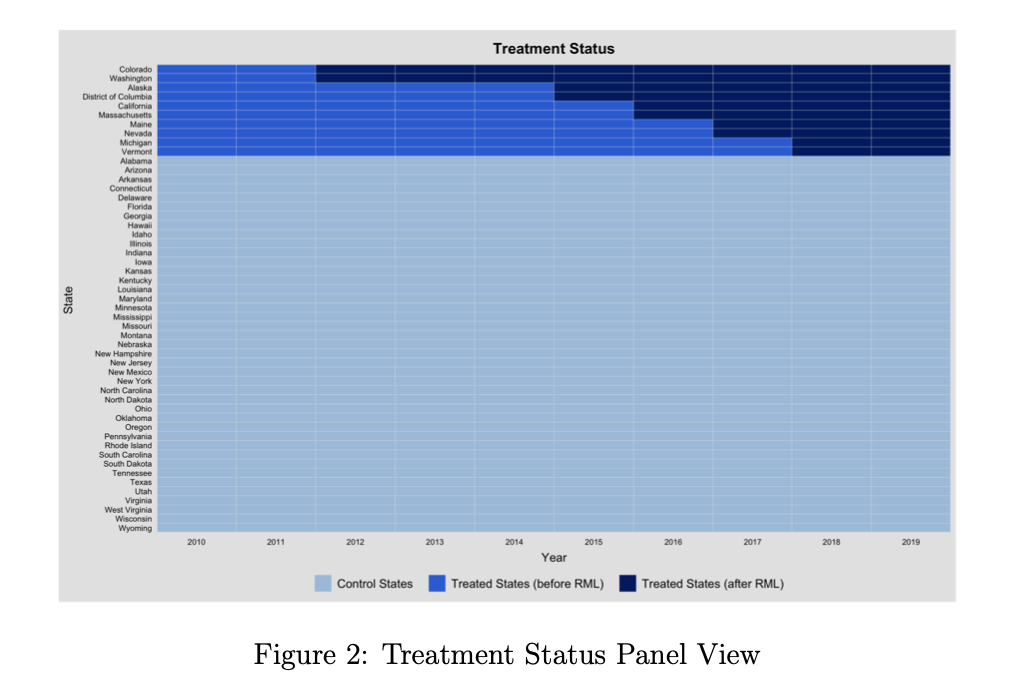
\includegraphics[scale = 0.33]{panel}

\end{frame}

\begin{frame} %Slide 5
\frametitle{Summary statistics}
	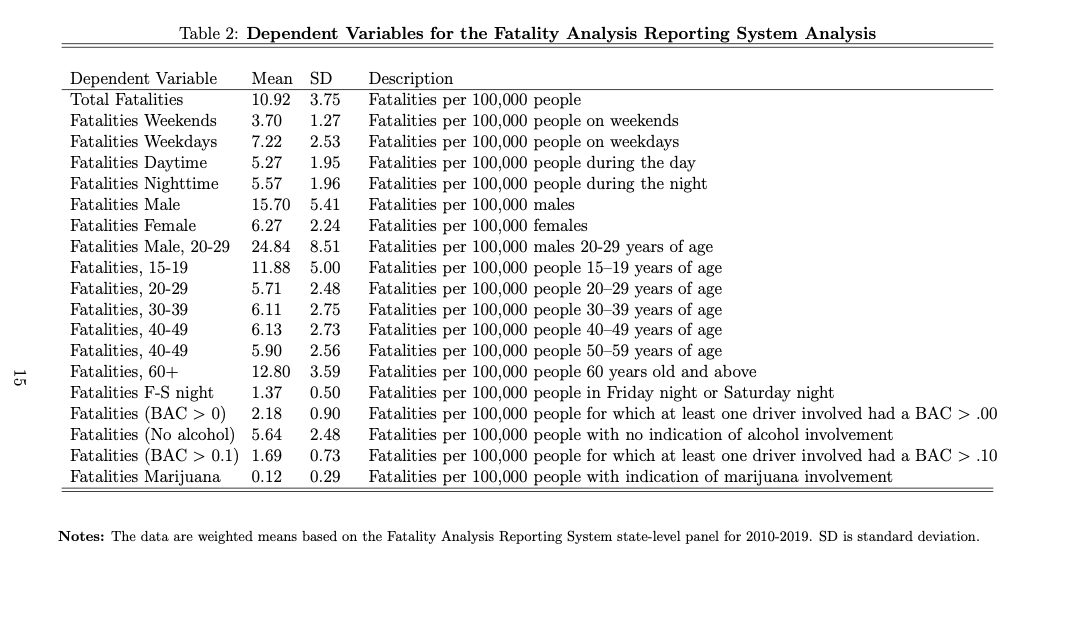
\includegraphics[scale = 0.33]{table2}

	
\end{frame}
\begin{frame} %Slide 6
\frametitle{Summary statistics}
	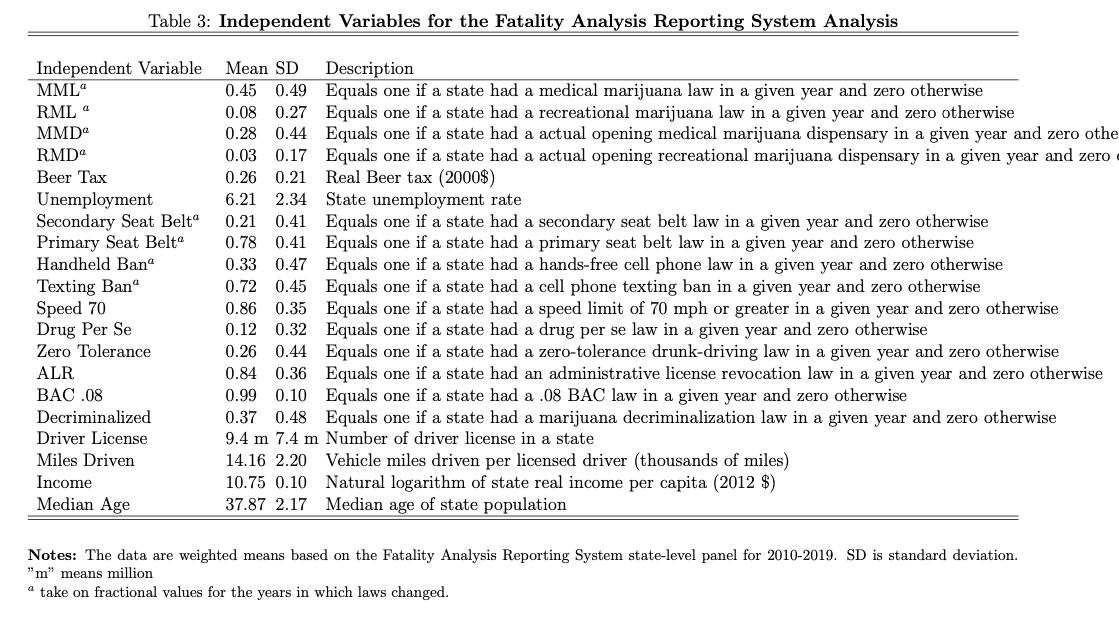
\includegraphics[scale = 0.33]{table3}

	
\end{frame}
\begin{frame} %Slide 6
\frametitle{Raw data- Trend in total fatalities}
	\includegraphics[scale = 0.13]{raw_fatal_rate.png}
\end{frame}

\begin{frame}
\frametitle{Regression Model} % Slide 7

$$ ln(traffic\_fatalities_{st}) = \beta_0 + \beta_1 MML_{st} + \alert{\beta_2} RML_{st} + X_{st} \beta_3 + \mu_s + \eta_t   +\epsilon_{st}$$

 $\alert{\beta_2}$  is a coefficient of interest. 

\end{frame}


\begin{frame} %Slide 8
\frametitle{Result}
	
	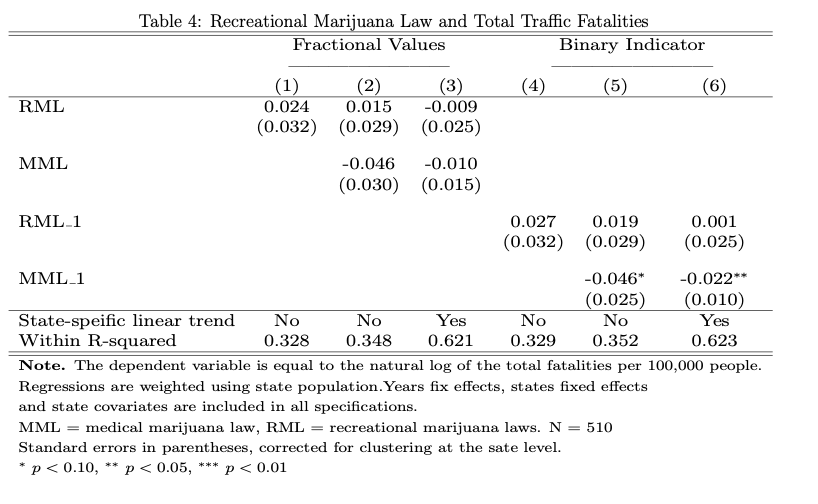
\includegraphics[scale = 0.33]{table4}
	
\end{frame}

\begin{frame} %Slide 9
\frametitle{Result}
	
	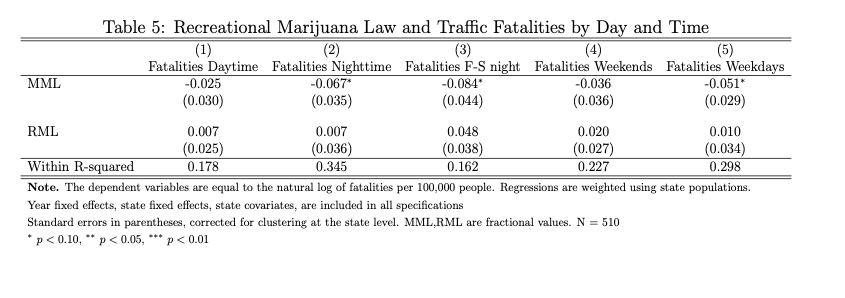
\includegraphics[scale = 0.33]{table5}
	
\end{frame}

\begin{frame} %Slide 10
\frametitle{Result}
	
	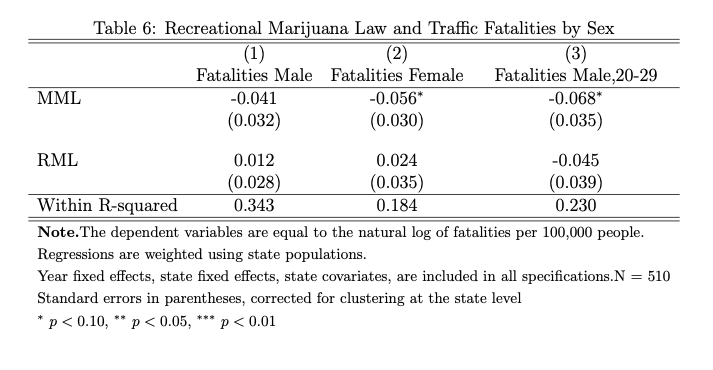
\includegraphics[scale = 0.33]{table6}
	
\end{frame}

\begin{frame} %Slide 11
\frametitle{Result}
	
	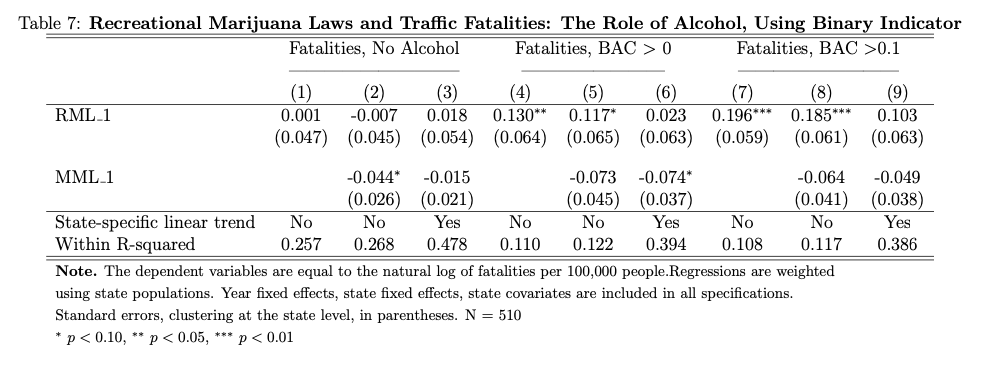
\includegraphics[scale = 0.33]{table7}
	
\end{frame}

\begin{frame} %Slide 12
\frametitle{Result}
	
	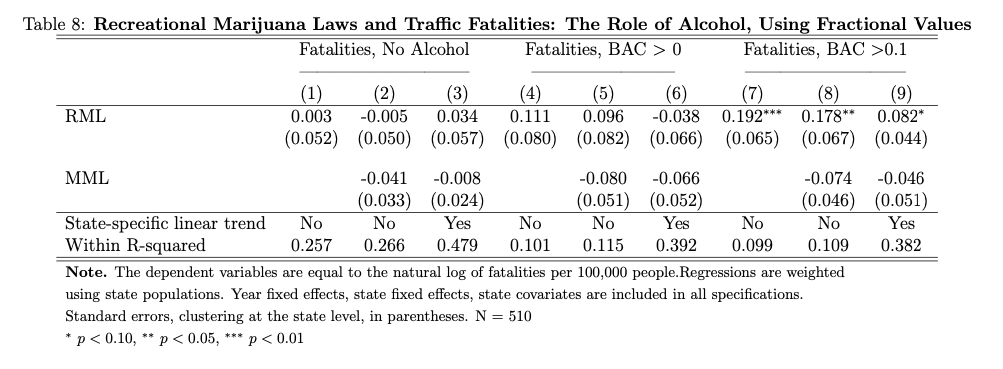
\includegraphics[scale = 0.33]{table8}
	
\end{frame}

\begin{frame} %Slide 13
\frametitle{Result- Event study}
	
	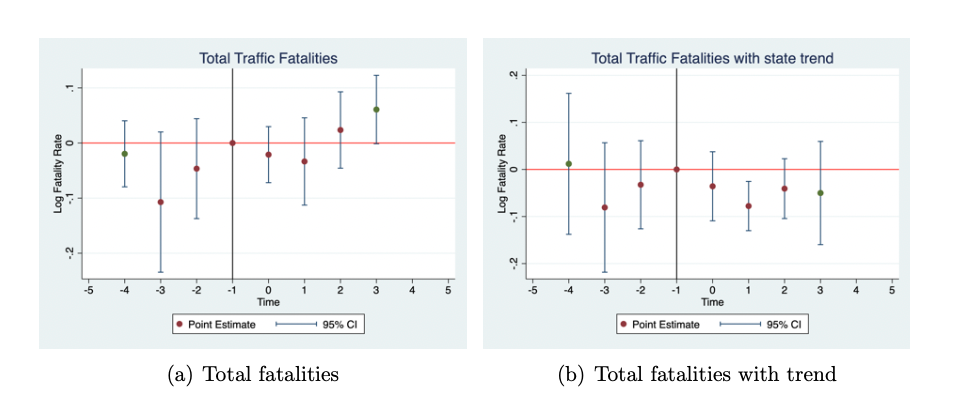
\includegraphics[scale = 0.33]{event1}
	
\end{frame}

\begin{frame} %Slide 14
\frametitle{Result- Event study}
	
	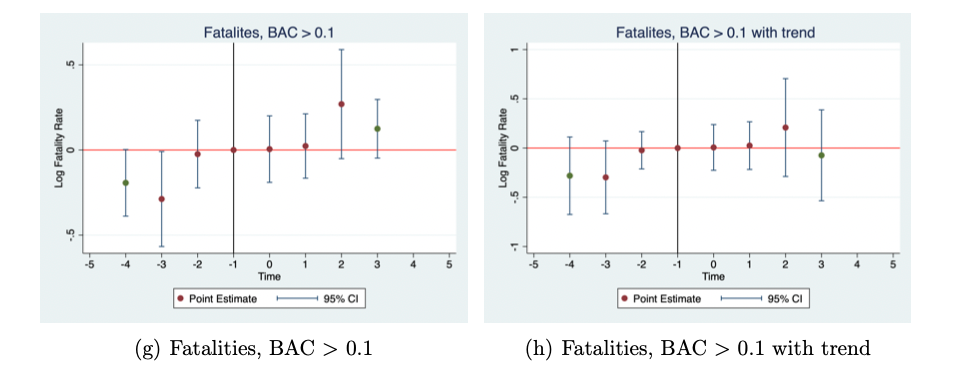
\includegraphics[scale = 0.33]{event2}
	
\end{frame}

\begin{frame}
\frametitle{TWFE concern?}
	\begin{enumerate}
		\item
	Goodman-Bacon(2021) shows that regular TWFE using early-adopting states as a counterfactual for later-adopting states will bias our estimates. \\ 
		\item
	Sun and Abraham(2020) claims that the evaluation of pre-treatment trends in event studies — as a test of common trends —unreliable  \\  
		\item
	In Andrew Baker blog, using recent econometric work on issues with TWFE staggered DiD designs to re-evaluate the effect of MMLs on opioid overdose mortality , he concluded "\alert{...it is unlikely that the adoption of medical marijuana laws and their timing was as-if random.Without real randomization we should be reluctant to make causal claims from staggered adoption alone.} " 
	\end{enumerate}
\end{frame}

\begin{frame} %Slide 11
\frametitle{Robustness checks - Bacon decomposition}
	
	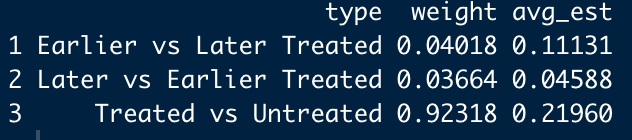
\includegraphics[scale = 0.5]{bacon}
	
\end{frame}

\begin{frame} %Slide 15
\frametitle{Result- Event study by Callaway- Sant'Anna(2018)}
	
	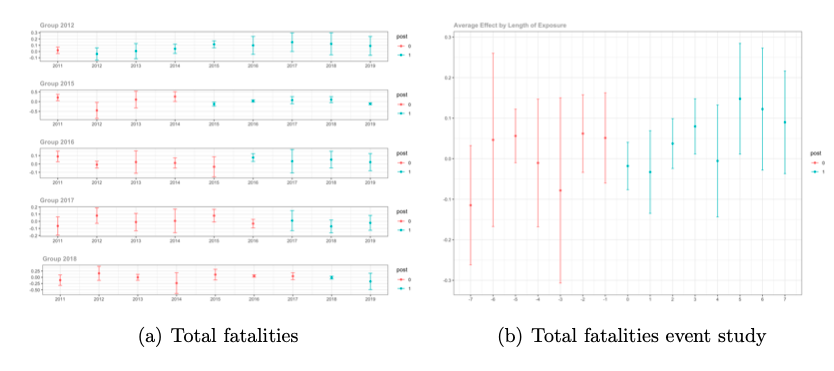
\includegraphics[scale = 0.33]{event3}
	
\end{frame}

\begin{frame} %Slide 16
\frametitle{Result- Event study by Callaway- Sant'Anna(2018)}
	
	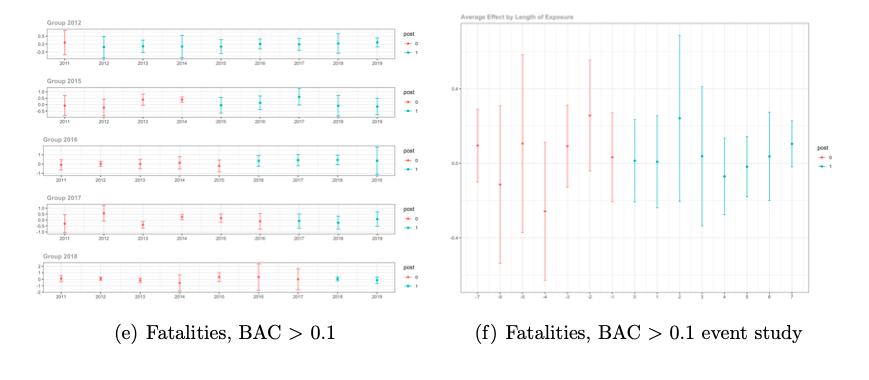
\includegraphics[scale = 0.33]{event4}
	
\end{frame}







\begin{frame} %Slide 11
\frametitle{Robustness checks- Selective Migration}
	Can't examine the composition of migration. 
	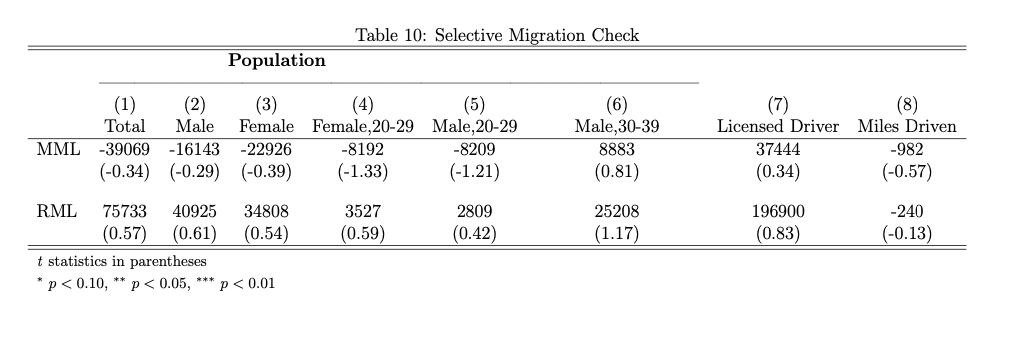
\includegraphics[scale = 0.33]{table10}
	
\end{frame}

\begin{frame} %Slide 11
\frametitle{Robustness checks - Using RMD and MMD}
	
	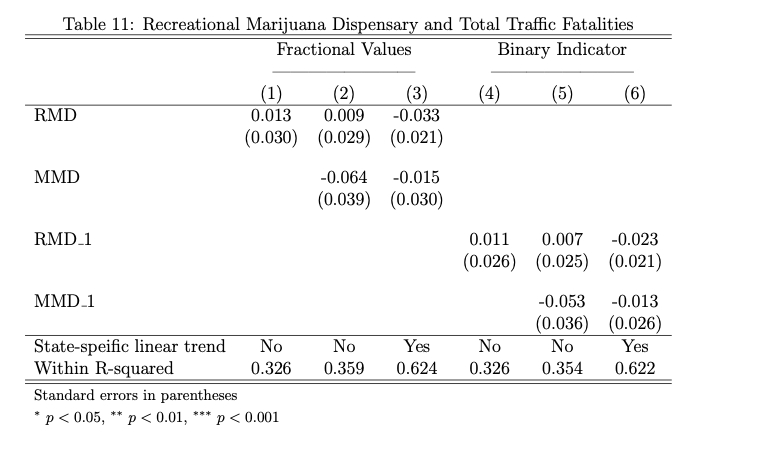
\includegraphics[scale = 0.33]{table11}
	
\end{frame}

\begin{frame} %Slide 
\frametitle{Robustness checks - Different definition of fatalities rate}
	
	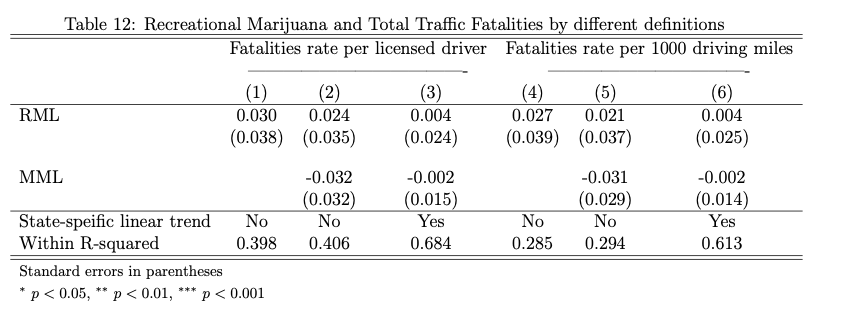
\includegraphics[scale = 0.33]{table12}
	
\end{frame}

\begin{frame} %Slide 
\frametitle{Robustness checks -Non DID model- Generalized Synthetic control by Yiqing Lu(2018)  }
		Required lots of pre-treatment data, it removes Colorado and Washington. 
	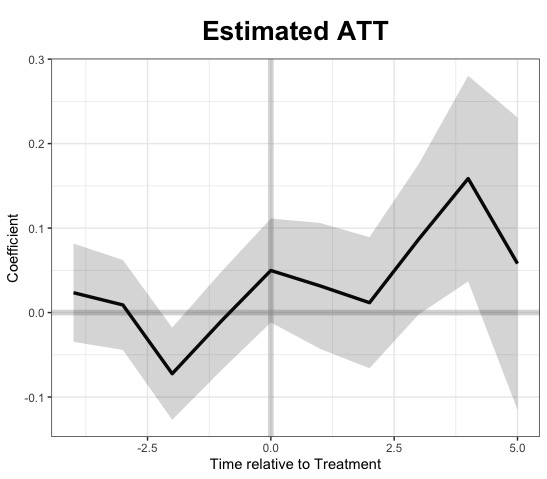
\includegraphics[scale = 0.38]{Generalized_synthetic}
\end{frame}


\begin{frame} %Slide 
\frametitle{Robustness checks -Non DID model- Counterfactual Estimator  by Licheng Liu(2021)}
	Total traffic fatalities

	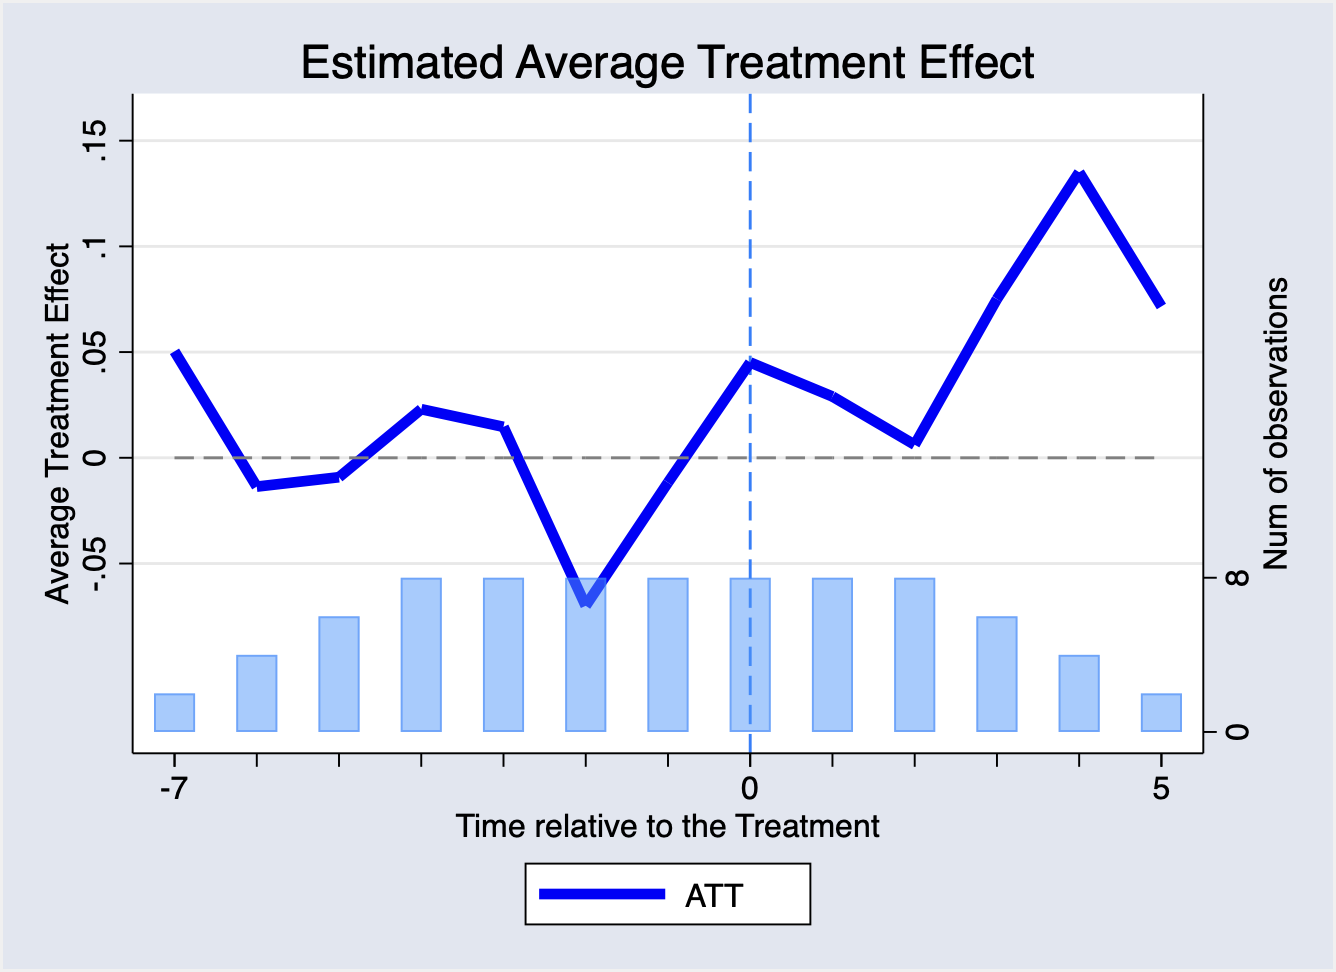
\includegraphics[scale = 0.38]{counter_estimator1} 	
\end{frame}

\begin{frame}
\frametitle{Disscusion and Conclusion- Potential limitation}
	\begin{enumerate}
		\item Can't check the composition of migration
		\item Lack of post-legalization data, so can't fully investigate the dynamic effect of RMLs
		
	
	\end{enumerate}


\end{frame}



\begin{frame}
\frametitle{Disscusion and Conclusion}
\begin{enumerate}
		\item
	Light evidence of positive effect  on total traffic fatalities, strong evidence of  large positive significant effect on alcohol-related traffic fatalities.$\implies$ Marijuana may not be a substitute of alcohol, contrary to many MML studies.  \pause
		\item
	Mechanism : selective migration, edible pot product, illegal-to-legal transformation. \pause
		\item
	Policy Implication: Combined with other studies, policy makers should be very careful when liberalizing the use of marijuana. \pause
		\item
	Future research: studies with more post-legalization data, studies taking advantages of natural experiment rather than only depending on TWFE mode to provide a causal claim. 
	\end{enumerate}
	
\end{frame}

\end{document}












